%\section{Training a Sentence Classifier without Alignment \label{sec:uschema}}
\section{Model \label{sec:model}}

\subsection {Universal Schema without Entity Embeddings}

While Compositional Universal Schema addresses reasoning over arbitrary textual patterns, it is still limited to reasoning over entity pairs seen at training time.
\citet{verga2015multilingual} approach this problem by using Universal Schema as a sentence classifier - directly comparing a textual relation to a kb relation to perform relation extraction.
However, this approach is unsatisfactory for two reasons.
The first is that this creates an inconsistency between training and testing, as the model is trained to predict compatibality between entity pairs and relations and not relations directly.
Secondly, it considers only a single piece of evidence while making its prediction.
The learned entity pair can be seen as a sumamrization of all relations for which that entity pair was seen.
\todo{describe that its uscham + aggregation - refer to figures}



\begin{figure}[h]
\caption{Aggragating relation type vectors to form entity pair vector}
\centering
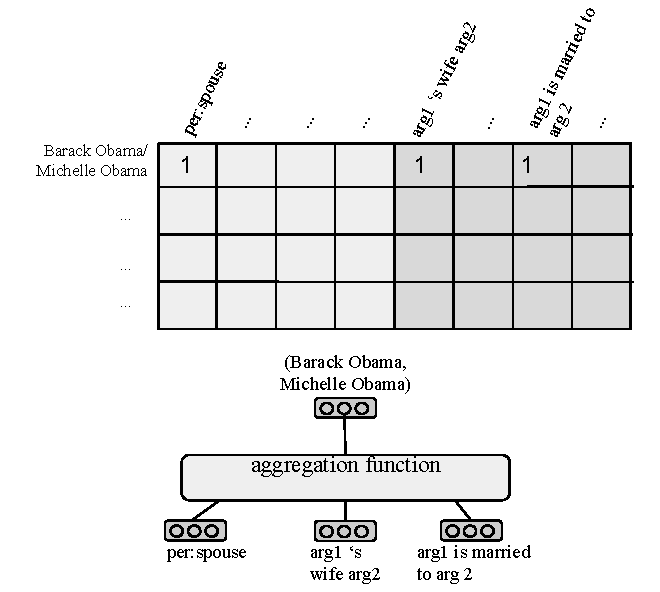
\includegraphics[scale=.68]{aggregate-entity}
\end{figure}


\subsection {Aggregation Functions}
In this work we examine several fairly simple aggregation functions.
\textbf{Mean Relation} creates a single centroid for the entity pair by averaging all of its relation vectors.
While this intuitive makes sense as an approximation for the explicit entity pair representation, averaging large numbers of embeddings can lead to a noisy signal.
The \textbf{Max Relation} represents the entity pair as its most similar relation to the query vector of interest.
This
 TopK Relations
 Dimension-wise Max Pool
   Convolution + Dimension-wise Max Pool
